\documentclass[10pt, letterpaper]{article}
\usepackage{graphicx}
\usepackage{amsmath}
\input{MyCommand}

\setlength{\topmargin}{-2cm}
\setlength{\oddsidemargin}{-0.3cm}
\setlength{\textheight}{23cm}
\setlength{\textwidth}{17cm}
\newtheorem{thm}{Theorem}

\newcommand{\pd}[2]{\frac{\partial #1}{\partial #2}}
\newcommand{\cint}[1]{\frac{1}{2\pi i}\oint_{#1}}
%\newcommand{\dfrac}[2]{\displaystyle\frac{#1}{#2}}

\begin{document}

\noindent
{\bf Exercises}
\begin{itemize}
	% --------------------------------------------------------------------------
	\item Ex. 1: 

	Define $u(x,y)$ and $v(x,y)$ as
	\be
		f(z) = \frac{xy^2(x+iy)}{x^2+y^2} = \frac{x^2y^2}{x^2+y^2} + i\frac{xy^3}{x^2+y^2} \equiv u(x,y) + iv(x,y),
	\ee
	where $z=x+iy$. By definition $z\neq 0$ and $f(0)=0$. It follows that
	\begin{align}
		\frac{\partial u}{\partial x} &= \frac{2xy^4}{(x^2+y^2)^2}, \nonumber\\
		\frac{\partial v}{\partial y} &= \frac{3x^3y^2+xy^4}{(x^2+y^2)^2}, \nonumber\\
		\frac{\partial u}{\partial y} &= \frac{2x^4y}{(x^2+y^2)^4}, \nonumber\\
		\frac{\partial v}{\partial x} &= \frac{y^5 - x^2y^3}{(x^2+y^2)^2}. \nonumber
	\end{align}
	Note that since $z\neq 0$ (i.e. $x$ and $y$ cannot be zero simultaneously), the denominators of the partial
	derivatives are all well defined. In order to satisfy the Cauchy-Riemann conditions, we only need to examine
	the numerators.
	\begin{itemize}
		\item Along the real-axis, $y=0$: In this case, $\partial u/\partial x = \partial v/\partial y=0$;
		$\partial u/\partial y = -\partial v/\partial x=0$. As a result, $f(z)$ is analytic and differentiable
		along the real-axis except $z=0$.
		\item Along the imaginary-axis, $x=0$: $\partial u/\partial x = \partial v/\partial y=0$. However,
		$\partial u/\partial y=0$, $-\partial v/\partial x = -y$. Therefore, $f(z)$ is not analytic nor differentiable
		on the imaginary-axis.
		\item For any $x, \,y\neq 0$, in order to satisfy the Cauchy-Riemann condition, we need to have
		\begin{align}
			2xy^4 &= 3x^3y^2 + xy^4, \label{eq:1}\\
			2x^4y &= x^2y^3 - y^5. \label{eq:2}
		\end{align}
		The first condition leads to $y^2 = 3x^2$. By substituting this identity into Eq.~(\ref{eq:2}), we get:
		\be
			x^4=0,
		\ee
		which contradicts to the condition that $x,\,y\neq 0$. Thus, $f(z)$ is not analytic nor differentiable
		for any finite $(x, y)$.
	\end{itemize}


	% --------------------------------------------------------------------------
	\item Ex. 6: 

	Given the definition $z=x+iy=re^{i\theta}$, we have $x=r\cos\theta$ and $y=r\sin\theta$.
	This transformation leads to
	\begin{align}
		\pd{x}{r} &= \cos\theta,\,\,\,\,\,\pd{x}{\theta}=-r\sin\theta,\nonumber\\
		\pd{y}{r} &= \sin\theta,\,\,\,\,\,\pd{y}{\theta}=r\cos\theta. \nonumber
	\end{align}
	It follows that
	\begin{align}
		\pd{u}{x} &= \pd{u}{r}\pd{r}{x} + \pd{u}{\theta}\pd{\theta}{x} 
		           = \frac{1}{\cos\theta}\pd{u}{r} - \frac{1}{r\sin\theta}\pd{u}{\theta},\nonumber\\
		\pd{v}{y} &= \pd{v}{r}\pd{r}{y} + \pd{v}{\theta}\pd{\theta}{y}
		           = \frac{1}{\sin\theta}\pd{v}{r} + \frac{1}{r\cos\theta}\pd{v}{\theta},\nonumber\\
		\pd{u}{y} &= \pd{u}{r}\pd{r}{y} + \pd{u}{\theta}\pd{\theta}{y}
		           = \frac{1}{\sin\theta}\pd{u}{r} + \frac{1}{r\cos\theta}\pd{u}{\theta},\nonumber\\
		\pd{v}{x} &= \pd{v}{r}\pd{r}{x} + \pd{v}{\theta}\pd{\theta}{x} 
		           = \frac{1}{\cos\theta}\pd{v}{r} - \frac{1}{r\sin\theta}\pd{v}{\theta}.\nonumber
	\end{align}
	With the above identities, the usual Cauchy-Riemann conditions in Cartesian coordinates
	\begin{align}
		\pd{u}{x} &= \pd{v}{y}, \nonumber\\
		\pd{v}{x} &= -\pd{u}{y},\nonumber
	\end{align}
	translate to
	\begin{align}
		\frac{1}{\cos\theta}\pd{u}{r} - \frac{1}{r\sin\theta}\pd{u}{\theta} &=
			\frac{1}{\sin\theta}\pd{v}{r} + \frac{1}{r\cos\theta}\pd{v}{\theta}, \label{eq:CR1}\\
		\frac{1}{\sin\theta}\pd{u}{r} + \frac{1}{r\cos\theta}\pd{u}{\theta} &=
			-\frac{1}{\cos\theta}\pd{v}{r} + \frac{1}{r\sin\theta}\pd{v}{\theta}. \label{eq:CR2}
	\end{align}
	Now, Eq.~(\ref{eq:CR1})$\times\sin\theta$ $-$ Eq.~(\ref{eq:CR2})$\times\cos\theta$ gives
	\be
		\pd{u}{r} = \frac{1}{r}\pd{v}{\theta}.
	\ee
	Similarly, Eq.~(\ref{eq:CR1})$\times\cos\theta$ $-$ Eq.~(\ref{eq:CR2})$\times\sin\theta$ leads to
	\be
		\pd{v}{r} = -\frac{1}{r}\pd{u}{\theta}.
	\ee

	% --------------------------------------------------------------------------
	\item Ex. 7:

	Firstly, let's write $z=re^{i\theta}$. 
	\begin{enumerate}
		\item $\log z$:

		With the definition of $z$ in polar form, we have
		\be
			\log z = \log r + i\theta \equiv u(r, \theta) + iv(r, \theta). \nonumber
		\ee
		It is straightforward to show that
		\begin{align}
			\pd{u}{r} &= \frac{1}{r} = \frac{1}{r}\pd{v}{\theta},\nonumber\\
			\pd{v}{r} &= 0 = -\frac{1}{r}\pd{u}{\theta}. \nonumber
		\end{align}

		\item $z^{1/2}$:
		\be
			z^{1/2} = r^{1/2} e^{i\theta/2} = r^{1/2}\cos\frac{\theta}{2} + ir^{1/2}\sin\frac{\theta}{2} 
			= u(r, \theta) + iv(r, \theta) \nonumber
		\ee
		Thus, following the definition of polar Cauchy-Riemann conditions:
		\begin{align}
			\pd{u}{r} &= \frac{1}{2}r^{-1/2}\cos\frac{\theta}{2} = \frac{1}{r}\pd{v}{\theta}, \nonumber\\
			\pd{v}{r} &= \frac{1}{2}r^{-1/2}\sin\frac{\theta}{2} = -\frac{1}{r}\pd{u}{\theta}. \nonumber
		\end{align}

		\item $z^{1/3}$:
		\be
			z^{1/3} = r^{1/3} e^{i\theta/3} = r^{1/3}\cos\frac{\theta}{3} + ir^{1/3}\sin\frac{\theta}{3} 
			= u(r, \theta) + iv(r, \theta) \nonumber
		\ee
		Thus
		\begin{align}
			\pd{u}{r} &= \frac{1}{3}r^{-2/3}\cos\frac{\theta}{3} = \frac{1}{r}\pd{v}{\theta}, \nonumber\\
			\pd{v}{r} &= \frac{1}{3}r^{-2/3}\sin\frac{\theta}{3} = -\frac{1}{r}\pd{u}{\theta}. \nonumber
		\end{align}		

	\end{enumerate}
	In all the three cases, $z\neq 0$, i.e. $r\neq 0$.

	% --------------------------------------------------------------------------
	\item Ex. 13:
	\begin{enumerate}
		\item $\tan(\tan^{-1}z) = z$

		Firstly, we have the following definitions:
		\begin{align}
			\tan z      &\equiv \frac{1}{i}\frac{e^{iz}-e^{-iz}}{e^{iz}+e^{-iz}} 
			            = \frac{1}{i}\frac{e^{2iz}-1}{e^{2iz}+1}, \nonumber\\
			\tan^{-1} z &\equiv \frac{i}{2}\ln\left(\frac{i+z}{i-z}\right). \nonumber
		\end{align}
		It follows that
		\be
			\exp\left(2i\cdot\frac{i}{2}\ln\left(\frac{i+z}{i-z}\right)\right)
			= \exp\left[-\ln\left(\frac{i+z}{i-z}\right)\right] \nonumber
			= \frac{i-z}{i+z}.
		\ee
		Therefore,
		\be
			\tan(\tan^{-1}z) = \frac{1}{i}\left(\frac{\dfrac{i-z}{i+z}-1}{\dfrac{i-z}{i+z}+1}\right) = z.
			\nonumber
		\ee

		\item $\log(e^z) = z + 2\pi ni$

		Write $z=re^{i\theta}$, we have
		\be
			e^z = e^{re^{i\theta}} = \underbrace{e^{r\cos\theta}}_{R}\cdot e^{i\overbrace{\scriptstyle r\sin\theta}^\phi} 
			    \equiv R\cdot e^{i\phi} \nonumber
		\ee
		With this identity, we can proceed to show that
		\be
			\log(e^z) = \log(R\cdot e^{i\phi}) = \log R + i\phi + 2\pi ni = r\cos\theta + ir\sin\theta + 2\pi ni = z + 2\pi ni.
			\nonumber
		\ee

	\end{enumerate}

	% --------------------------------------------------------------------------
	\item Ex. 15:
	The complex function $\tanh z$ is defined as follows
	\be
		\tanh z = \frac{e^z  - e^{-z}}{e^z + e^{-z}} = \frac{e^{2z} - 1}{e^{2z} + 1}.
	\ee
	To determine the singularities of $\tanh z$, we look at the second form. Namely, the function is singular if the denominator
	is zero or equivalently:
	\be
		e^{2z} = -1.
	\ee
	This condition is satisified if $2z = \pm i (2n+1)\pi$ where $n=0, 1, 2, \ldots$. As a result, $\tanh z$ is singular if
	$z$ satisifies
	\be
		z = \pm i \left(n + \frac 1 2 \right)\pi.
	\ee



	% --------------------------------------------------------------------------
	\item Ex. 16:

	Between the following integrals
	\be
		\mbox{a)}\,\,\,\int_{-1}^1 z^* dz,\hspace{1.5cm}
		\mbox{b)}\,\,\,\int_0^i\sin 2z dz, \nonumber
	\ee
	the first integral does not make sense because $z^*$ is not analytic anywhere in the complex plane. Thus the value of
	a) depends on the path of integration. In the textbook, it is already shown that along a unit circle $C$,
	\be
		\oint_C z^* dz = 2\pi i. \nonumber
	\ee
	Using this result, a) can be viewed as going from $x=-1$ to $x=1$ along either the {\it upper} unit circle or 
	the {\it lower} unit circle, which gives the result of $-i\pi$ and $i\pi$ respectively. Moreover, if we just plug in
	the definition of $z=x+iy$ and recognize that along the real axis $y=0$, $dy=0$, we get
	\be
		\int_{-1}^i z^* dz = \int_{-1}^1 x\,dx = 0. \nonumber
	\ee
	All these results just demonstrate that the integral in a) really is path-dependent.

	It could be concluded that the integral in b) makes sense, and now we proceed to evaluate the integral.
	Using the definition $z=x+iy$ and the complex sine function, we have
	\be
		\sin 2z\,dz = (\cosh 2y\sin 2x\,dx - \sinh 2y\cos 2x\,dy) + i(\cosh 2y\sin 2x\,dy + \sinh 2y\cos 2x\,dx) 
		\label{eq:ex16integrand}
	\ee
	Since $x=0$ and $dx=0$ along the $y$-axis, it follows that
	\be
		\int_0^i\sin 2z\,dz = \int_0^1 -\sinh 2y\,dy = \frac{1}{2}(1-\cosh 2). 
		\label{ex16:direct_integral}
	\ee

	Instead of taking the path from the origin to $(x,y)=(0,1)$ along the imaginary axis, we could compute the integral
	from the origin to $(x,y)=(1,0)$ along the real axis ($OA$), then from $(1,0)$ to $(1,0)$ along the line $y=1-x$ ($AB$).
	Let's do this.

	On the first path $y=0$ and $dy=0$. So the integrand Eq.~(\ref{eq:ex16integrand}) becomes $\sin 2x$, thus
	\be
		\int_{OA} \sin 2z\,dz = \int_0^1\sin 2x\,dx  = \frac{1}{2}(1-\cos 2). \nonumber
	\ee

	Going from $(1,0)$ to $(0,1)$, we have $y=1-x$. This leads to
	\begin{align}
		\int_{AB} \sin 2z\,dz
			=& \int_{AB} (\cosh 2y\sin 2x\,dx - \sinh 2y\cos 2x\,dy) + 
			   i\int_{AB} (\cosh 2y\sin 2x\,dy + \sinh 2y\cos 2x\,dx) \nonumber\\
			=& -\int_0^1 (\cosh 2y\sin 2(1-y)\,dy + \sinh 2y\cos 2(1-y)\,dy) \nonumber \\
			 & + i\int_0^1 (\cosh 2y\sin 2(1-y)\,dy - \sinh 2y\cos 2(1-y)\,dy) \nonumber\\
			=& -\frac{1}{2}\left[\vphantom{\int} \cosh 2y \cos 2(1-y)\right]_0^1 
			   + \frac{i}{2}\left[\vphantom{\int} \sinh2y \sin 2(1-y)\right]_0^1 \nonumber\\
			=& \frac{1}{2}(\cos 2 - \cosh 2). \nonumber
	\end{align}

	Finally,
	\be
		\int_0^i\sin 2z\,dz = \int_{OA}\sin 2z\,dz + \int_{AB}\sin 2z\,dz = \frac{1}{2}(1-\cosh 2),
	\ee
	in agreement with Eq.~(\ref{ex16:direct_integral}) as expected.

	% --------------------------------------------------------------------------
	\item Ex. 18:
	\begin{enumerate}
		\item Since $C$ is a closed contour containing $z_0$, we write $f(z) = z^4 + 2z + 1$ and the integral can then
		be evaluated in the canonical form:
		\be
			I = \oint_C \frac{f(z)}{(z-z_0)^4}dz = \frac{2\pi i}{3!} f^{(3)}(z_0) = \frac{2\pi i}{3!}\times 24 z_0 = 8\pi i z_0.
			\nonumber
		\ee

		\item Because $C$ is a closed contour containing the origin, we invoke the canonical formula:
		\be
			I = \oint_C \frac{\cosh z}{z^{n+1}}dz = \left.\frac{2\pi i}{n!}\frac{d^n}{dz^n}\cosh z\right|_{z=0}
			\nonumber
		\ee
		The derivative on the right hand side is
		\be
			\left.\frac{d^n}{dz^n}\cosh z\right|_{z=0} = 
			\left\{
				\begin{array}{cc}
				\left.\sinh z\right|_{z=0}=0,         & n=1, 3, 5, \ldots\\ \\
				\left.\cosh z\right|_{z=0}=\frac 1 2, & n=0, 2, 4, \ldots
				\end{array}
			\right.
			\nonumber
		\ee
		By combining the two cases, we arrive at
		\be
			I = \frac{2\pi i}{n!}\frac{[1 + (-1)^n]}{2}. \nonumber
		\ee

	\end{enumerate}

	% --------------------------------------------------------------------------
	\item Ex. 19:
	Following the hint, we consider the integral
	\be
		I = \frac{1}{2\pi i}\oint_C \frac{P(z) - P(a)}{z-a}dz,
		\label{ex19}
	\ee
	where $C$ is a contour enclosing the point $a$. Since the numerator is analytic, $I$ can be evaluated by
	directly invoking Cauchy's integral formula. Namely:
	\be
		I = [P(z) - P(a)]_{z=a} = 0. \nonumber
	\ee
	However, we can also express the right hand side of Eq.~(\ref{ex19}) as follows:
	\be
		I = \frac{1}{2\pi i}\oint_C \frac{P(z) - P(a)}{z-a}dz = \frac{1}{2\pi i}\oint_C \frac{P(z)}{z-a}dz 
			- P(a)\cdot\frac{1}{2\pi i}\oint_C \frac{1}{z-a}dz.
		\nonumber
	\ee
	The second integral is just $P(a)$ by Cauchy's integral formula. Thus we arrive at
	\be
		\frac{1}{2\pi i}\oint_C \frac{P(z)}{z-a}dz = P(a).
	\ee
	The is a welcoming result which shows that Cauchy's integral formula can also be applied to complex
	polynomials.


	% --------------------------------------------------------------------------
	\begin{figure}
	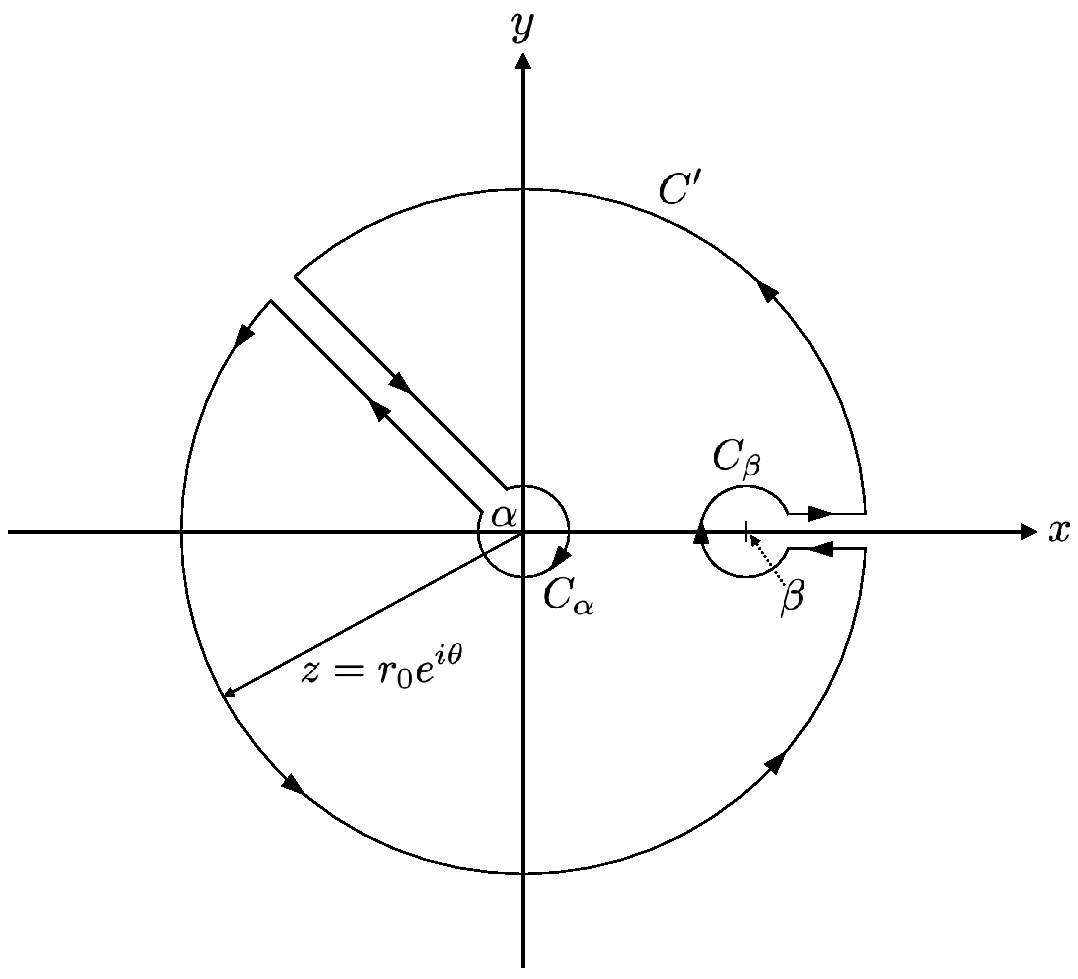
\includegraphics[width=0.45\textwidth]{./figures/fig_ex20.pdf}
	\caption{Contour for Exercise 20.}
	\label{fig:ex20}
	\end{figure}

	\item Ex. 20:
	We'd like to evaluate the following contour integral for an analytic function $f(z)$:
	\be
		I = \frac{1}{2\pi i}\oint_C \frac{f(z)}{(z-\alpha)(z-\beta)}dz, \nonumber
	\ee
	where $\alpha$ and $\beta$ are two distinct arbitrary points inside the contour $C$. We can choose $C$
	to be a circle such that $\alpha$ is the center of $C$ and $z=r_0 e^{i\theta}$, as shown in Fig.~\ref{fig:ex20}.
	In the figure, we choose the axis so that $\alpha$ and $\beta$ lie on the real axis. However, this arrangement
	is really not necessary. 

	In any case, we can add two circles $C_\alpha$ and $C_\beta$ around $\alpha$ and $\beta$ respectively, along
	with two sets of opposite-traversing line segments joining the inner circles with $C$. Let's call the contour
	as $C'$. Then we can write
	\be
		\cint{C'}\frac{f(z)}{(z-\alpha)(z-\beta)}dz = 
			I + \cint{C_\alpha}\frac{f(z)}{(z-\alpha)(z-\beta)}dz
			  + \cint{C_\beta}\frac{f(z)}{(z-\alpha)(z-\beta)}dz. \nonumber
	\ee
	The integral along $C'$ vanishes because now the integrand is analytic within the contour $C'$
	For the second term on the right-hand side, we notice that the term 
	\be
		\frac{f(z)}{z-\beta} \nonumber
	\ee
	is analytic within $C_\alpha$, so the integral is given immediately by Cauchy's integral formula:
	\be
		\cint{C_\alpha}\frac{f(z)}{(z-\alpha)(z-\beta)}dz = -\frac{f(\alpha)}{\alpha-\beta}. \nonumber
	\ee
	Similarly for the last term, we have
	\be
		\cint{C_\beta}\frac{f(z)}{(z-\alpha)(z-\beta)}dz = -\frac{f(\beta)}{\beta-\alpha}. \nonumber
	\ee
	Therefore, it follows that
	\be
		\cint{C}\frac{f(z)}{(z-\alpha)(z-\beta)}dz = \frac{f(\alpha) - f(\beta)}{\alpha-\beta}.
		\label{eq:ex20}
	\ee

	In order to deduce the Liouville's Theorem, we take Eq.~(\ref{eq:ex20}) and rewrite it as:
	\be
		f(\alpha) - f(\beta) = \frac{\alpha - \beta}{2\pi i}\oint_C \frac{f(z)}{(z-\alpha)(z-\beta)}dz. \nonumber
	\ee
	Now consider the norm of the left-hand side:
	\begin{align}
		\left|f(\alpha) - f(\beta)\right| 
			&= \frac{|\alpha - \beta|}{2\pi}\left| \oint_C \frac{f(z)}{(z-\alpha)(z-\beta)}dz \right| \nonumber\\
			&\leq \frac{|\alpha - \beta|}{2\pi} \oint_C \frac{|f(z)|}{|z-\alpha||z-\beta|}|dz|. \nonumber
	\end{align}
	By construction, $|z-\alpha| = r_0$, and $|dz|=r_0d\theta$. By assumption $f(z)$ is bounded, so $|f(z)| \leq M$.
	We can also choose the radius of $C$ such that $|z-\beta| \geq r_0/2$, for example. Then it follows that
	\be
		|f(\alpha) - f(\beta)| 
			\leq \frac{|\alpha - \beta|}{2\pi r_0} \frac{2M}{r_0}2\pi r_0
			= \frac {2|\alpha - \beta|}{r_0}M. \nonumber
	\ee
	We can choose the radius of $C$ arbitarrily large, the right hand side of the above inequality tends to be zero
	as $r_0\rightarrow\infty$. Thus
	\be
		|f(\alpha) - f(\beta)| = 0.
	\ee
	This result implies that $f(\alpha)=f(\beta)$ for arbitrary $\alpha$ and $\beta$. Thus $f(z)=\mbox{const.}$


\end{itemize}

\end{document}